\documentclass{ximera}

\author{Anna Davis} \title{MTH 160 Homework 3} 

\begin{document}

\begin{abstract}

\end{abstract}
\maketitle
 \textit{Certificate due: 9/9/2020 at 11:59 p.m.}
 \section{Lectures 5 and 6}
\begin{problem}\label{prob:160hom3prob1}
For each given function $g$, identify the "base function" $f$, and select the transformations applied to the graph of $f$ to obtain the graph of $g$.
\begin{enumerate}
    \item $g(x)=-x^2+1$
    
    Base function:  $f(x)=\answer{x^2}$
    \begin{multipleChoice}  
\choice{Reflection about the $x$-axis; Horizontal shift to the right by 1 unit.}
\choice[correct]{Reflection about the $x$-axis; Vertical shift up by 1 unit.}  
\choice{Reflection about the $y$-axis; Vertical shift down by 1 unit.}  
\choice{Horizontal shift to the left by 1 unit.}  
\end{multipleChoice}
\item $g(x)=\frac{1}{x}+2$
    
    Base function:  $f(x)=\answer{\frac{1}{x}}$
    \begin{multipleChoice}  
\choice{Horizontal shift to the right by 2 units.}
\choice{Horizontal shift to the left by 2 units.}
\choice[correct]{Vertical shift upwards by 2 units.}  
\choice{Vertical shift downwards by 2 units.}  
  \end{multipleChoice}
  \item $g(x)=\sqrt{x+3}-1$
    
    Base function:  $f(x)=\answer{\sqrt{x}}$
    \begin{multipleChoice}  
    \choice{Vertical shift upwards by 3 units; Vertical shift downwards by 1 unit.}  
\choice{Horizontal shift to the right by 3 units; Vertical shift downwards by 1 unit.}
\choice{Horizontal shift to the left by 3 units; Vertical shift upwards by 1 unit.}
\choice[correct]{Horizontal shift to the left by 3 units; Vertical shift downwards by 1 unit.}  
  \end{multipleChoice}
  \item $g(x)=-\frac{1}{x-4}$
    
    Base function:  $f(x)=\answer{\frac{1}{x}}$
    \begin{multipleChoice}  
 \choice[correct]{Horizontal shift to the right by 4 units; Reflection about the $x$-axis.}
\choice{Horizontal shift to the left by 4 units; Reflection about the $x$-axis.}
\choice{Vertical shift upwards by 4 units; Reflection about the $x$-axis.} 
\choice{Reflection about the $y$-axis.  Vertical shift downwards by 4 units.}  
  \end{multipleChoice}
\end{enumerate}
\end{problem}
\begin{problem}\label{prob:160hom3prob2}
The graphs of function $f$ (in red) and function $g$ (in blue) are given. Express $g$ in terms of $f$.
\begin{enumerate}
    \item \begin{image}
   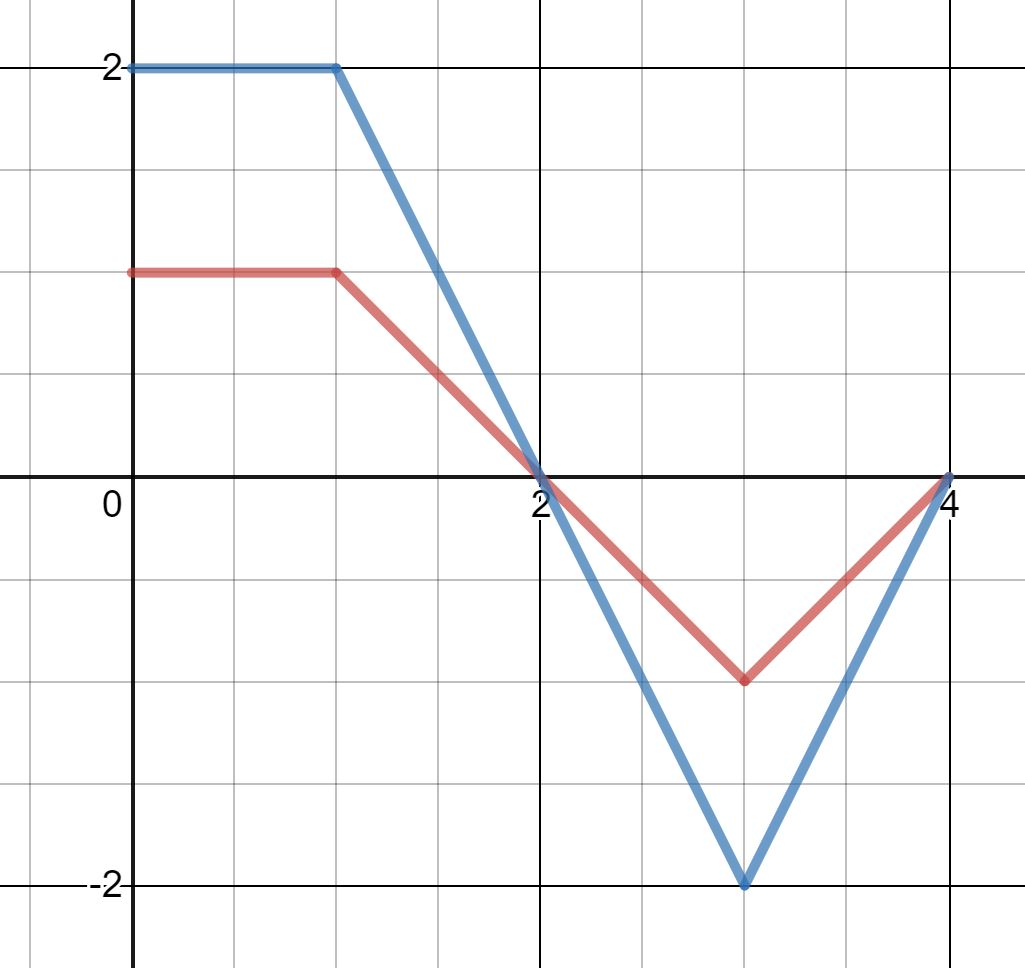
\includegraphics[height=1in]{160H3pic4.jpg}
 \end{image}
 \begin{multipleChoice}  
 \choice[correct]{$g(x)=2f(x)$}
\choice{$g(x)=f(x)+2$}
\choice{$g(x)=f(x-2)$} 
\choice{$g(x)=f(x+2)$}  
  \end{multipleChoice}
  
   \item \begin{image}
   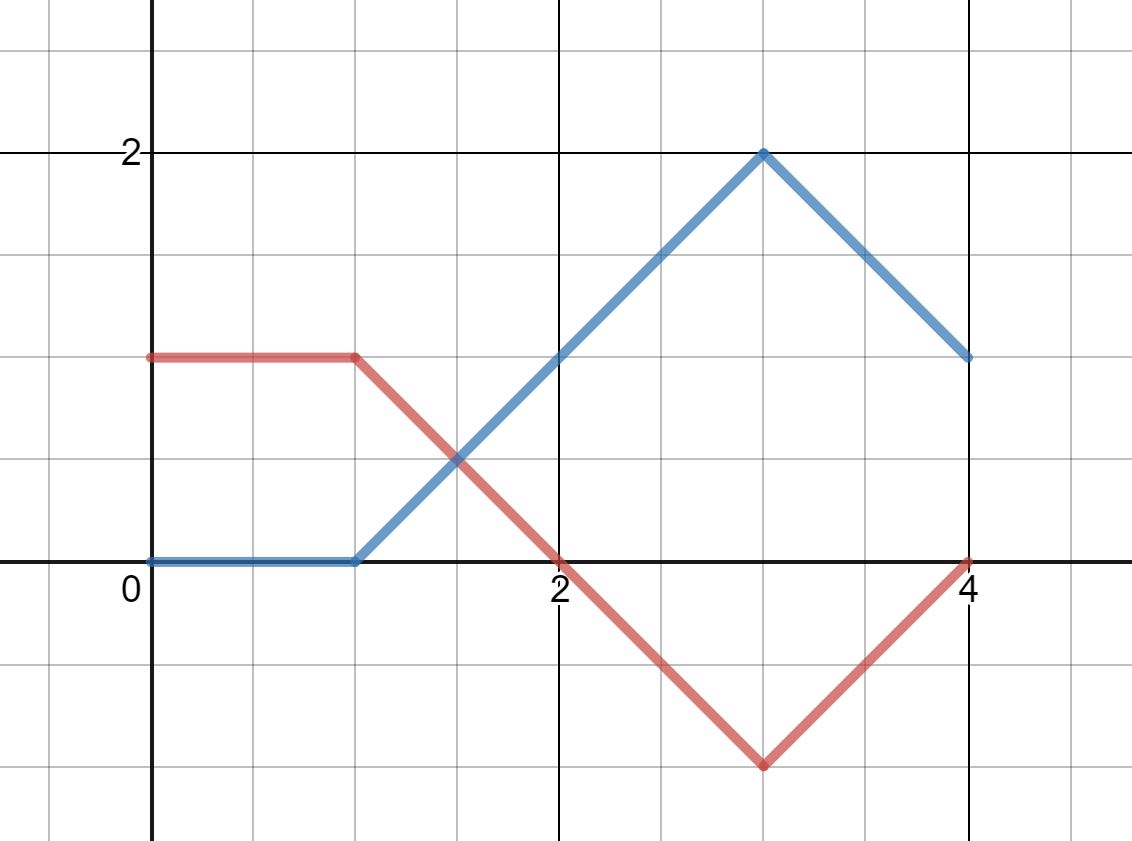
\includegraphics[height=1in]{160H3pic2.jpg}
 \end{image}
 \begin{multipleChoice}  
 \choice{$g(x)=-f(x)-1$}
\choice{$g(x)=-f(x-1)$} 
\choice{$g(x)=-f(x+1)$}  
\choice[correct]{$g(x)=-f(x)+1$}
  \end{multipleChoice}
  
  \item \begin{image}
   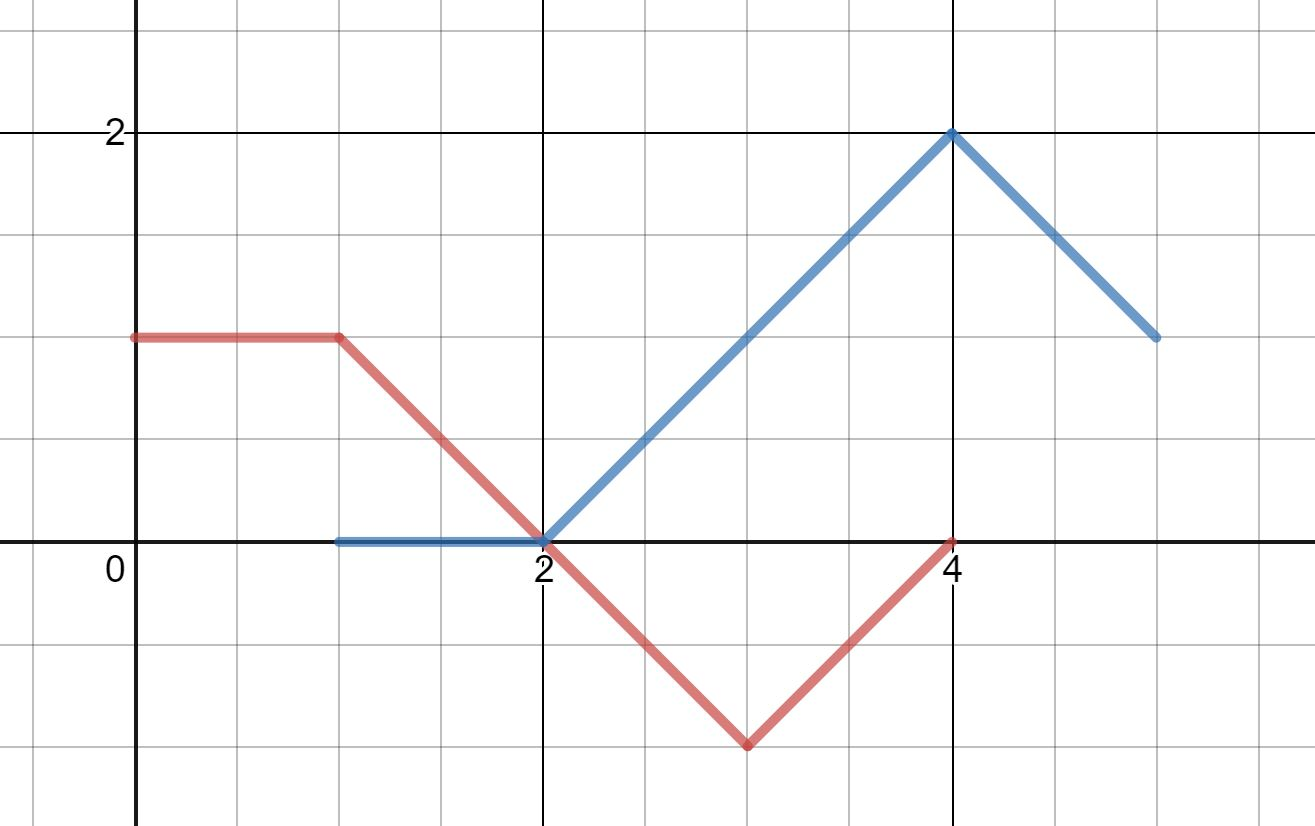
\includegraphics[height=1in]{160H3pic3.jpg}
 \end{image}
 \begin{multipleChoice}  
 \choice{$g(x)=-f(x+1)-1$}
 \choice[correct]{$g(x)=-f(x-1)+1$}
\choice{$g(x)=-f(x-1)-1$} 
\choice{$g(x)=f(x+1)$}  
  \end{multipleChoice}
\end{enumerate}
\end{problem}
\section{Lecture 7}
\begin{problem}\label{prob:160hom3prob3}
The graph of a function and its inverse are shown below.  
\begin{image}
   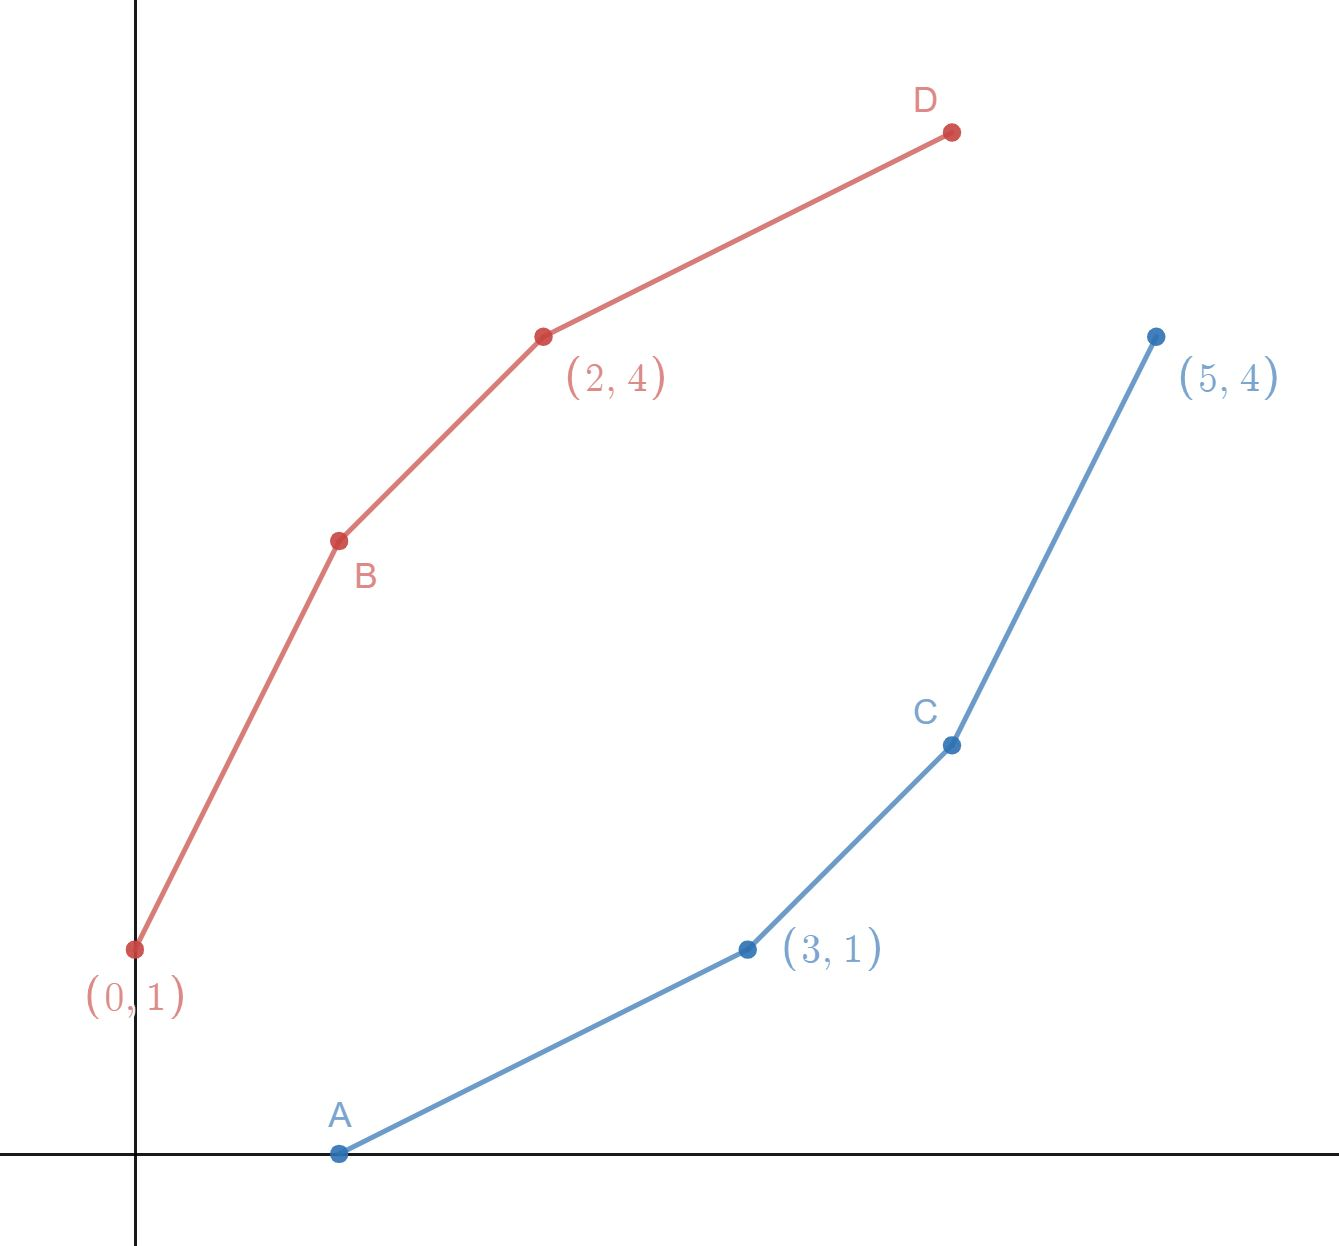
\includegraphics[height=1in]{160H3pic1.jpg}
 \end{image}
Find the coordinates of $A, B, C, D$.
$$A=(\answer{1},\answer{0}),\quad B=(\answer{1},\answer{3}),\quad C=(\answer{4},\answer{2}),\quad D=(\answer{4},\answer{5})$$
The two graphs are symmetric about the line
$y=\answer{x}$.
\end{problem}
\begin{problem}\label{prob:160hom3prob4}
Find $f^{-1}$.
\begin{enumerate}
    \item $f(x)=5x+7$
    $$f^{-1}(x)=\answer{\frac{1}{5}}x-\answer{\frac{7}{5}}$$
    \item $f(x)=\frac{1}{x+10}$
    $$f^{-1}(x)=\answer{\frac{1}{x}-10}$$
\end{enumerate}

\end{problem}
\end{document} 